
\begin{enumerate}
    \item A particle is moved along a path AB-BC-CD-DE-EF-FA, as shown in figure, in presence of a force $\vec{F} = (\alpha y t + 2 \alpha x) N$, where $x$ and $y$ are in meter and $\alpha = -1 Nm^{-1}$. The work done on the particle by this force $\vec{F}$ will be \_\_\_\_\_\_\_ Joule.
    
\begin{center}
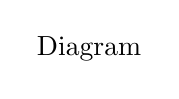
\begin{tikzpicture}
\node {Diagram};
\end{tikzpicture}
\end{center}
    
\end{enumerate}
